% Compelling argument demonstrating success criteria met, or well-justified explanation of different direction taken.

% Excellent critical thought and interpretation which substantiate any claims of success.

\label{sec:4}

\section{Review of Success Criteria}
\label{sec:review-of-success-criteria}
My project has met all success criteria as outlined below:

\begin{enumerate}[font=\bfseries]
    \item[1a.]\textbf{Multiple agents will be able to localize themselves within a world using purely visual data.} \\
    My system is the first decentralized SLAM system capable of operating using only monocular camera data. This removes the need for large and expensive stereo camera, LiDAR or RGBD sensors.

    \item[1b.]\textbf{Agents will be capable of communicating with each other to build a shared understanding of the world.} \\
    Agents use ROS to perform decentralized and reliable communication with eachother, and are able to merge maps and share key frames to build a shared world.

    \item[1c.]\textbf{Agents will be able to act independently, failing gracefully if it loses communication with its peers.} \\
    Agents fall back to performing single-agent visual SLAM when communication with their peers is degraded or lost. Once communication is regained, the agents share their unsent map data.

    \item[2.]\textbf{Evaluate the capabilities of the system compared to a comparable single-agent system.} \\
    This is done in the \nameref{sec:benchmarking} Section. I go beyond the original success criteria by also comparing my system to comparable multi-agent systems, demonstrating my system's superior performance.

\end{enumerate}


After discussions with my supervisor, we decided to not pursue my original project extensions, instead focusing on deploying the SLAM system on physical robots and building... TODO

\section{Benchmarking}
\label{sec:benchmarking}
This section will benchmark the performance of my system when run on industry standard visual SLAM datasets. All evaluations are run using only monocular camera data.

The Central Management Interface is used to stream the dataset to the agents and my library \textit{Multi Agent EVO} is used to provide the Absolute Trajectory Error (ATE).

\subsection{EuRoC Machine Hall}
\label{sec:euroc-machine-hall}
The EuRoC Machine Hall dataset \autocite{burri2016euroc} is one of the most widely used visual SLAM datasets, providing a 752x480 20fps video feed and millimeter level ground truth data at 20hz. The camera rig is attached to a Micro Aerial Vehicle (MAV) which flies through a large machine room. To simulate a multi-agent dataset, we run the Machine Hall 01-03 scenarios in parallel on three agents.

All three agents merge initialize maps of vastly different scales but are able to merge within XXX seconds and begin sharing map data.

\autoref{fig:euroc-mh-01-03-line-plot} shows the ATE of my system when running this dataset. The overall RMS ATE is only 6.2cm over the 279m total trajectory length, demonstrating my system's very impressive accuracy. It is clear that my system is performing SLAM as opposed to simple visual odometry as the ATE returns back to the baseline at the end of each run when the agents return back to their starting position.

\begin{figure}[h]
    \centering
    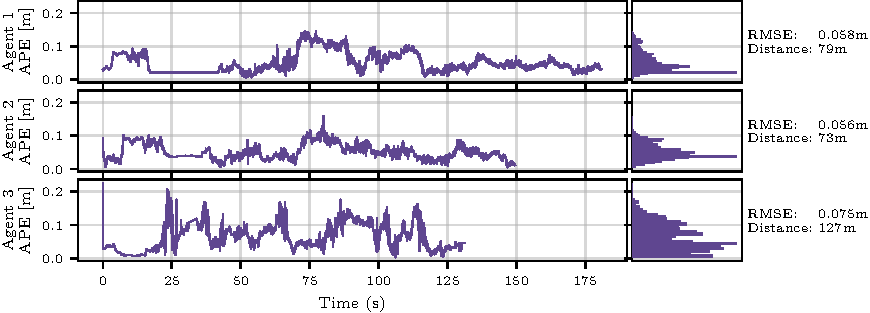
\includegraphics[width=\linewidth]{figures/EuRoC_MH_01-03_line_plot.pdf}

    \caption{Plot of my system's average trajectory error (ATE) with respect to the ground truth when running the EuRoC Machine Hall 01-03 scenarios in parallel on three agents. The average RMSE of the multi-agent system is 0.062m over the 279m total trajectory length. \captionbreak RMSE represents the root mean square of the ATE.}
    \label{fig:euroc-mh-01-03-line-plot}
\end{figure}

TODO do a plot of like 5 runs to show low variance.

We now run the Machine Hall 01 and 02 scenarios on two agents to analyze the network usage in \autoref{fig:euroc-mh-01-02-bandwith}. Initially, the agents send bag of word information before quickly detecing a merge opportunity. Agent 1 then procedes to send its full map to agent 2, which can be seen as a large initial spike in network bandwith. The agents successfully merge, and begin exchanging key frames. The rate of key frame data being sent rises and falls depending on how much new area the agent is exploring.

Along with sending key frames, the agents sporadically send map points to refine their map alignment. This occurs less frequently the longer system runs due to the additive increase multiplicative decrease method used to schedule map alignments, described in the \nameref{sec:map-alignment-refiner} Section. However, the size of the messages also grows over time due to the larger number of tracked map points.

The total data exchanged by the two agent system is 55.7MB over 184 seconds, giving an average communication rate of 302.6KB/s. 84\% of this is from key frame data, which is sent at an average of 127KB/s by each agent.

\begin{figure}[h]
    \centering
    \begin{subfigure}[b]{0.55\linewidth}
        \centering
        \marginbox{0 0 0 0} {
            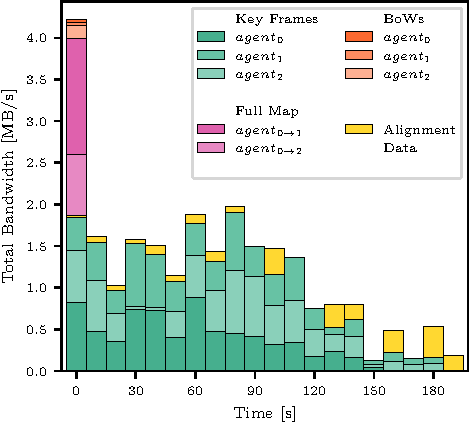
\includegraphics[width=\linewidth, valign=t]{figures/apr11_mh_trajectory_b_bandwith.pdf}
        }
        \caption{Total system data over time}
    \end{subfigure}%
    ~
    \begin{subfigure}[b]{0.45\linewidth}
        \flushright
        \adjustbox{valign=t, width=\linewidth}{
            \marginbox{0.2in 0 0 0} {

                \def\arraystretch{1.2}
                \begin{tabular}{ |c|l|r|r| }
                    \cline{3-4}
                    \multicolumn{2}{}{}                       & \multicolumn{1}{|c|}{KB} & \multicolumn{1}{|c|}{Avg. KB/s}         \\
                    \hline
                    \multirow{3}{*}{Key Frames}               & $agent_0$                & 69,971                          & 351.9 \\
                                                              & $agent_1$                & 63,908                          & 321.4 \\
                                                              & $agent_2$                & 65,164                          & 327.7 \\
                    \hline
                    \multirow{3}{*}{BoWs}                     & $agent_0$                & 371                             & 1.9   \\
                                                              & $agent_1$                & 437                             & 2.2   \\
                                                              & $agent_2$                & 1,496                           & 7.5   \\
                    \hline
                    \multirow{2}{*}{Full Map}
                                                              & $agent_{0\to1}$          & 13,953                          & 70.2  \\
                                                              & $agent_{0\to2}$          & 7,319                           & 36.8  \\
                    \hline
                    \multicolumn{2}{|c|}{Alignment Data}      & 22,560                   & 113.6                                   \\
                    \hline
                    \multicolumn{2}{|c|}{\textbf{Total Data}} & \textbf{245,218}         & \textbf{1,233.1}                        \\
                    \hline
                \end{tabular}
            }
        }
        \caption{Total system data by message type}
        \vfill

        \adjustbox{valign=b, width=\linewidth}{
            \marginbox{0.2in 0 0 0.3in} {
                \def\arraystretch{1.2}
                \begin{tabular}{ |l|r|r|r|r| }
                    \cline{2-5}
                    \multicolumn{1}{}{} & \multicolumn{2}{|c|}{Sent} & \multicolumn{2}{|c|}{Received}                                                               \\
                    \cline{2-5}
                    \multicolumn{1}{}{} & \multicolumn{1}{|c|}{KB}   & \multicolumn{1}{|c|}{Avg. KB/s} & \multicolumn{1}{|c|}{KB} & \multicolumn{1}{|c|}{Avg. KB/s} \\
                    \hline
                    $agent_0$           & \textbf{114,585}           & \textbf{576.2}                  & \textbf{131,005}         & \textbf{658.8}                  \\
                    \hline
                    $agent_1$           & \textbf{64,345}            & \textbf{323.6}                  & \textbf{173,554}         & \textbf{872.8}                  \\
                    \hline
                    $agent_2$           & \textbf{66,660}            & \textbf{335.2}                  & \textbf{164,606}         & \textbf{827.7}                  \\
                    \hline
                \end{tabular}
            }
        }
        \caption{Data by agent}
    \end{subfigure}%

    \caption{Bandwidth used by the EuRoC Machine Hall 01-03 scenarios running on my SLAM system.}
    \label{fig:euroc-mh-01-02-bandwith}
\end{figure}

\subsection{TUM-VI Rooms}
\label{sec:tum-rooms}
The TUM visual-intertial dataset \autocite{8593419} consists of handheld fisheye 512x512 video with ground truth data. As before, we use only monocular visual data and combine the room1-3 sessions to simulate a multi-agent dataset. The "room" environment is used for this evaluation, which is a motion capture lab with plain flat walls with some posters hung up. There is less texture in this environment than the machine hall, making visual-only SLAM more difficult. Additionally, parts of the room are revisited dozens of times by different agents, allowing us to evaluate our system's ability to relocalize agents within previously mapped environments.


\begin{figure}[h]
    \centering
    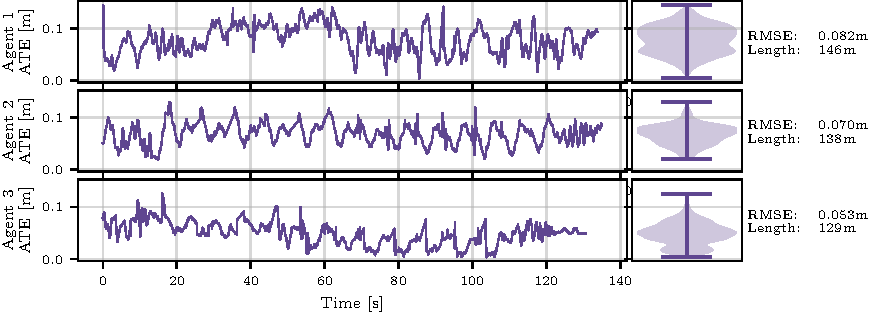
\includegraphics[width=\linewidth]{figures/apr11_tum_room_trajectory_a_line_plot.pdf}

    \caption{Plot of my system's average trajectory error (ATE) with respect to the ground truth when running the EuRoC Machine Hall 01-03 scenarios in parallel on three agents. The average RMSE of the multi-agent system is 0.062m over the 279m total trajectory length. \captionbreak RMSE represents the root mean square of the ATE.}
    \label{fig:euroc-mh-01-03-line-plot}
\end{figure}

\begin{figure}[h]
    \centering
    \begin{subfigure}[b]{0.55\linewidth}
        \centering
        \marginbox{0 0 0 0} {
            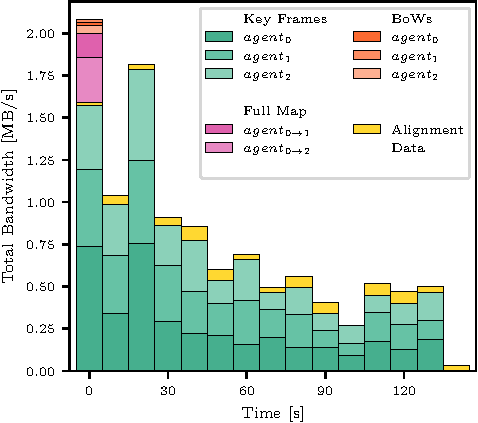
\includegraphics[width=\linewidth, valign=t]{figures/apr11_tum_room_trajectory_a_bandwith.pdf}
        }
        \caption{Total system data over time}
    \end{subfigure}%
    ~
    \begin{subfigure}[b]{0.45\linewidth}
        \flushright
        \adjustbox{valign=t, width=\linewidth}{
            \marginbox{0.2in 0 0 0} {

                \def\arraystretch{1.2}
                \begin{tabular}{ |c|l|r|r| }
                    \cline{3-4}
                    \multicolumn{2}{}{}                       & \multicolumn{1}{|c|}{KB} & \multicolumn{1}{|c|}{Avg. KB/s}         \\
                    \hline
                    \multirow{3}{*}{Key Frames}               & $agent_0$                & 37,599                          & 264.9 \\
                                                              & $agent_1$                & 33,066                          & 233.0 \\
                                                              & $agent_2$                & 29,963                          & 211.1 \\
                    \hline
                    \multirow{3}{*}{BoWs}                     & $agent_0$                & 217                             & 1.5   \\
                                                              & $agent_1$                & 188                             & 1.3   \\
                                                              & $agent_2$                & 426                             & 3.0   \\
                    \hline
                    \multirow{2}{*}{Full Map}
                                                              & $agent_{0\to1}$          & 1,472                           & 10.4  \\
                                                              & $agent_{0\to2}$          & 2,631                           & 18.5  \\
                    \hline
                    \multicolumn{2}{|c|}{Alignment Data}      & 6,947                    & 49.0                                    \\
                    \hline
                    \multicolumn{2}{|c|}{\textbf{Total Data}} & \textbf{112,511}         & \textbf{792.8}                          \\
                    \hline
                \end{tabular}
            }
        }
        \caption{Total system data by message type}
        \vfill

        \adjustbox{valign=b, width=\linewidth}{
            \marginbox{0.2in 0 0 0.3in} {
                \def\arraystretch{1.2}
                \begin{tabular}{ |l|r|r|r|r| }
                    \cline{2-5}
                    \multicolumn{1}{}{} & \multicolumn{2}{|c|}{Sent} & \multicolumn{2}{|c|}{Received}                                                               \\
                    \cline{2-5}
                    \multicolumn{1}{}{} & \multicolumn{1}{|c|}{KB}   & \multicolumn{1}{|c|}{Avg. KB/s} & \multicolumn{1}{|c|}{KB} & \multicolumn{1}{|c|}{Avg. KB/s} \\
                    \hline
                    $agent_0$           & \textbf{49,083}            & \textbf{345.9}                  & \textbf{63,644}          & \textbf{448.5}                  \\
                    \hline
                    $agent_1$           & \textbf{33,254}            & \textbf{234.3}                  & \textbf{76,624}          & \textbf{539.9}                  \\
                    \hline
                    $agent_2$           & \textbf{30,389}            & \textbf{214.1}                  & \textbf{80,649}          & \textbf{568.3}                  \\
                    \hline
                \end{tabular}
            }
        }
        \caption{Data by agent}
    \end{subfigure}%

    \caption{Bandwidth used by the TUM-VI Rooms 01-03 scenarios running on my SLAM system.}
    \label{fig:euroc-mh-01-02-bandwith}
\end{figure}

%evaluate how

\section{Comparison to Related Work}
\label{sec:comparison-to-related-work}

% compare to ccm slam, and also vins mono with multisession running which is shit lol.

% compare data transfer with covins and ccm-slam which is shit

% Qualitative and quantitative


\section{Real World Experiments}
\label{sec:real-world-experiments}
Deploying my system on physical robots demonstrates its ability to be run in real time within the computational, bandwith and latency constraints of real world systems. Furthermore, it demonstrates the robustness of my development framework which allowed seamless migration from local testing using simulations to a real distributed system using live camera feeds with no changes to my code base.

The details of the real world setup are given in the \nameref{sec:real-world-implementation} Section. In summary, the Cambridge RoboMasters platform was used

\subsection{Multi-Agent Collision Avoidance}
\label{sec:multi-agent-collision-avoidance}
In this experiment, we showcase the NMPC collision avoidence motion controller working in conjunction with the SLAM system to avoid collisions with both static and dynamic obstacles. Real time relative position data from the SLAM system is fed to the NMPC collision avoidance motion controller which controls the robot's velocity accordingly.



